% `advanced_example.tex', an advanced example employing the AIAA class
% plus other third-party LaTeX packages.
%
% For a bare-bones usage, see `template.tex'.
%
% Typical processing for PostScript (PS) output:
%
%  latex advanced_example
%  bibtex advanced_example  (bibliography)
%  makeindex -s nomencl.ist -o advanced_example.gls advanced_example.glo
%                            (nomenclature)
%  latex advanced_example   (repeat as needed to resolve references)
%
%  xdvi advanced_example    (onscreen draft display)
%  dvips advanced_example   (postscript)
%  gv advanced_example.ps   (onscreen display)
%  lpr advanced_example.ps  (hardcopy)
%
% With the above, only Encapsulated PostScript (EPS) images can be used.
%
%
%  pdflatex advanced_example
%  bibtex advanced_example    (bibliography)
%  makeindex -s nomencl.ist -o advanced_example.gls advanced_example.glo
%                              (nomenclature)
%  pdflatex advanced_example  (repeat as needed to resolve references)
%
%  acroread advanced_example.pdf  (onscreen display)
%
% If you have EPS figures, you will need to use the epstopdf script
% to convert them to PDF because PDF is a limmited subset of EPS.
% pdflatex accepts a variety of other image formats such as JPG, TIFF,
% PNG, and so forth -- check the documentation for your version.
%
% If you do *not* specify suffixes when using the graphicx package's
% \includegraphics command, latex and pdflatex will automatically select
% the appropriate figure format from those available.  This allows you
% to produce PS and PDF output from the same LaTeX source file.
%
% To generate a large format (e.g., 11"x17") PostScript copy for editing
% purposes, use
%
%  dvips -x 1467 -O -0.65in,0.85in -t tabloid advanced_example
%
% For further details and support, read the Users Manual, aiaa.pdf.

\documentclass[]{aiaa-tc}% insert '[draft]' option to show overfull boxes

 \usepackage{varioref}%  smart page, figure, table, and equation referencing
 \usepackage{wrapfig}%   wrap figures/tables in text (i.e., Di Vinci style)
 \usepackage{threeparttable}% tables with footnotes
 \usepackage{dcolumn}%   decimal-aligned tabular math columns
  \newcolumntype{d}{D{.}{.}{-1}}
 \usepackage{nomencl}%   nomenclature generation via makeindex
  \makeglossary
 \usepackage{amssymb,amsmath}
 \usepackage{subfigure}% subcaptions for subfigures
 \usepackage{subfigmat}% matrices of similar subfigures, aka small mulitples
 \usepackage{fancyvrb}%  extended verbatim environments
 \fvset{fontsize=\footnotesize,xleftmargin=2em}
 \usepackage{lettrine}%  dropped capital letter at beginning of paragraph
%  \usepackage[dvips]{dropping}% alternative dropped capital package
 \usepackage[colorlinks]{hyperref}%  hyperlinks [must be loaded after dropping]
 \usepackage{float}
 \usepackage{longtable,booktabs,tabularx}
 % \restylefloat{table}
 \usepackage{graphicx}
 \usepackage{caption}
 \usepackage{siunitx}
 \usepackage{multicol}
 \usepackage{indentfirst}
 \usepackage{environ}
 \usepackage[labelfont=bf]{caption}
 \usepackage{multirow}
 \usepackage{setspace}
%  \graphicspath{{./figs/}}
 \usepackage[sort, numbers]{natbib}

\usepackage{bm}
%\title{Conceptual Design of an Extremely Short Takeoff and Landing Aircraft (using GPkit/for Urban Air Mobility)}
\title{Feasibility Study of Short Takeoff and Landing Urban Air Mobility Vehicles using Geometric Programming}
 \author{
  Chris Courtin\thanks{Graduate Student, Aeronautics and Astronautics Engineering, MIT, 77 Mass Ave, Cambridge MA, 02139, AIAA Member.}, 
  Michael Burton\thanks{Graduate Student, Aeronautics and Astronautics Engineering, MIT, 77 Mass Ave, Cambridge MA, 02139, AIAA Student.}, 
  Patrick Butler\thanks{Graduate Student, Aeronautics and Astronautics Engineering, MIT, 77 Mass Ave, Cambridge MA, 02139, AIAA Student.}, 
  Alison Yu\thanks{Graduate Student, Aeronautics and Astronautics Engineering, MIT, 77 Mass Ave, Cambridge MA, 02139, AIAA Student.}, 
 Parker Vascik \thanks{Graduate Student, Aeronautics and Astronautics Engineering, MIT, 77 Mass Ave, Cambridge MA, 02139, AIAA Student.}, 
  John Hansman\thanks{T. Wilson Professor, Aeronautics and Astronautics Engineering, MIT, 77 Mass Ave, Cambridge MA, 02139, AIAA Member.} \\
  {\normalsize\itshape
   Massachusetts Institute of Technology, Cambridge, 02139, USA}\\
 }

 % Data used by 'handcarry' option
 \AIAApapernumber{YEAR-NUMBER}
 \AIAAconference{Conference Name, Date, and Location}
 \AIAAcopyright{\AIAAcopyrightD{YEAR}}

 % Define commands to assure consistent treatment throughout document
 \newcommand{\eqnref}[1]{(\ref{#1})}
 \newcommand{\class}[1]{\texttt{#1}}
 \newcommand{\package}[1]{\texttt{#1}}
 \newcommand{\file}[1]{\texttt{#1}}
 \newcommand{\BibTeX}{\textsc{Bib}\TeX}
 \usepackage{hyperref}
 \hypersetup{citecolor = blue}

\begin{document}

\graphicspath{{./figs/}}
\maketitle

\begin{abstract}
    The feasibility of an Urban Air Mobility (UAM) system that features electric Extremely Short Takeoff and Landing (ESTOL) vehicles is investigated.  An overview is given of the system constraints that must be incorporated into the design of the vehicle.  The system-wide advantages and limitations of ESTOL aircraft are discussed, for both near- and far-term system implementations.  A detailed vehicle sizing model is developed using geometric programming, a robust optimization framework.  This model is used to determine feasible boundaries on required runway size, vehicle range, and the sensitivity of the vehicle design to high-level mission parameters such as speed and number of passengers.  Key unique drivers of the vehicle design are identified.  The impact of distributed electric propulsion (DEP) is assessed.  Performance relative to a comparable Vertical Takeoff and Landing (VTOL) vehicle is analyzed, both with currently available technology and forecasted future technology.   The infrastructure requirements (runway size, approach paths, etc.) needed to support ESTOL operations are assessed according to current regulations.  Two major urban areas (Boston and Los Angeles) are presented as case studies to show where this infrastructure could be feasibly located.  Key challenges and risks to implementation are discussed.  


\end{abstract}

\section*{Nomenclature}

\begin{multicols}{2}
\small

\begin{tabbing}
  XXXXXXX \= \kill% this line sets tab stop
$A$ \> takeoff helper variable \\
$AR$ \> wing aspect ratio \\
$b$ \> wing span \\ % [ft] \\
$B$ \> takeoff helper variable \\
$c$ \> wing chord \\ %[m] \\
$C_D$ \> drag coefficient \\
$CDA$ \> area drag coefficient \\
$C_{D_g}$ \> ground drag coefficient \\
$c_{d_p}$ \> wing profile drag coefficient \\
$C_L$ \> lift coefficient \\
$C_{L_g}$ \> ground lift coefficient \\
$C_{L_{\mathrm{max}}}$ \> max lift coefficient \\
$D$ \> drag \\
$e$ \> span efficiency \\
$f_{\mathrm{struct}}$ \> fractional structural weight \\
$g$ \> gravitational constant \\
$L$ \> lift \\
$\mathcal{M}_{\mathrm{root}}$ \> root moment stress \\
$N$ \> deceleration factor \\
$P_{\mathrm{shaft-max}}$ \> max shaft power \\
$P_{\mathrm{spec}}$ \> specific motor power \\
$Re$ \> Reynolds number \\
$S$ \> wing area \\
$S_{\mathrm{land}}$ \> landing ground roll \\
$S_{\mathrm{runway}}$ \> runway distance \\
$S_{\mathrm{TO}}$ \> take off ground roll \\
$S_{y_{\mathrm{spar}}}$ \> spar section modulus \\
$t$ \> time \\
$T$ \> thrust \\
$V$ \> speed \\
$V_{\mathrm{stall}}$ \> stall speed \\
$W_{\mathrm{batt}}$ \> battery weight \\
$W_{\mathrm{fadd}}$ \> additional wing weight\\
$W_{\mathrm{motor}}$ \> motor weight \\
$W_{\mathrm{MTO}}$ \> max take off weight \\
$W_{\mathrm{pay}}$ \> payload weight \\
$W_{\mathrm{skin}}$ \> wing skin weight \\
$W_{\mathrm{spar}}$ \> wing spar weight \\
$W_{\mathrm{struct}}$ \> structural weight \\
$W_{\mathrm{wing}}$ \> wing weight \\
$\eta_{\mathrm{elec}}$ \> combined electric efficiency \\
$\eta_{\mathrm{prop}}$ \> propeller efficiency \\
$\mu$ \> rolling friction coefficient \\
$\rho$ \> air density \\
$\sigma_{\mathrm{CFRP}}$ \> carbon fiber allowable stress \\
 \end{tabbing}

\end{multicols}
% \printglossary% creates nomenclature section produced by MakeIndex

\section{Introduction}
Within the aviation industry there is a strong and growing interest in the development of Urban Air Mobility (UAM) networks,  which are aerial transportation systems in and around major metropolitan areas.  The defining features of UAM networks are fleets of relatively small vehicles operating off a distributed network of takeoff and landing areas (TOLAs) located within dense urban centers, primarily focused on passenger transport. Past efforts at developing UAM networks based on helicopters were largely unsuccessful due to the high costs of helicopter operation, the high levels of noise generated during operations, and the poor safety record of these aircraft~\cite{Vascik2017}.  Recent advances in electric vehicle propulsion and key subsystem technologies have opened the door to new vehicle configurations that may mitigate these fundamental challenges.  The ride-sharing operational models that have been successfully developed for ground transportation also have the potential to improve the economics of UAM  operations through pooling and on-demand service. This has sparked renewed interest in the UAM concept, and there are currently over a dozen legacy and emerging aircraft manufacturers building or flight-testing UAM-specific aircraft. 

All of the UAM vehicles currently under development utilize an all-electric power train and have vertical takeoff and landing (VTOL) capability; they are commonly known as eVTOL aircraft.  Within this eVTOL landscape, there are many different proposed configurations, including tilt-rotors, multicopters, slowed rotors, and tilt-wings.  Almost all configurations are also based on the concept of distributed electric propulsion (DEP), which replaces one or two large helicopter-style rotors with many small rotors.  These DEP eVTOL configurations have several advantages;  VTOL capability minimizes the amount of space required at TOLAs and susceptibility to crosswinds, while DEP increases system efficiency and safety while reducing mechanical complexity and, potentially, cost and noise.  This is useful capability for operations in noise-sensitive areas where takeoff and landing space is at a premium, but it also imposes two significant penalties on the vehicle.  The first is in performance; the weight of the high-power system needed to perform the vertical takeoff and landing limits the amount of payload these vehicles can carry, or the range at which they can carry it.  This effect is especially pronounced for electric aircraft, where payload and range are already compromised by the poor specific energy of current battery technology relative to hydrocarbon fuels.  The second and more significant penalty is that VTOL configurations increase the already substantial amount of risk associated with the UAM concept.  

Any proposed UAM system is exposed to many sources of risk, such as local noise regulations, ATC capacity concerns, pilot or automation availability, infrastructure availability, and uncertain market demand~\cite{Vascik2017}~\cite{Uber}.  Of all the risk sources, however, the most significant is whether, and within what timeframe, it will be possible to certify these new types of aircraft.  This risk is so significant for two reasons.  It is highly likely to be a factor - historically, certification of new aviation technologies is a slow and difficult process -  and it is highly consequential.  The inability to certify a vehicle would preclude any type of UAM operations.

In considering certification risk, it is important to differentiate between risk inherent in certifying a vehicle configuration, and risk inherent in certifying a vehicle flight control system.  In many UAM proposals, advanced vehicle automation is seen as a key enabling technology for large-scale operations, while initial operations are expected to operate with a human pilot operating the aircraft ~\cite{Uber}.  To achieve that initial operational capability, only certification of vehicle automation or flight control systems required by the configuration for piloted operations (such as the flight stabilization system in a multicopter) should be considered.  Certification of advanced autonomous systems is a separate risk category, and should not be confused the risk of certifying the vehicle configuration for traditional piloted operations. 

Certification risk arises from the potential for catastrophic vehicle failures, whether or not the catastrophic failure modes are sufficiently mitigated, and how complex the mitigations required are.  A vehicle with few inherent catastrophic failure modes is easier to certify than a vehicle where many catastrophic failure modes are mitigated by a variety of complex systems.  For DEP eVTOL aircraft, certification risk arises from the potential failure of three critical systems common to all configurations:  1) the active flight stabilization system that controls vehicle attitude and lift during the vertical and translational phases of flight via differential thrust 2) the power delivery system that supplies power from the batteries to the motors, and the motors themselves and 3) the batteries that store electrical power. 

Total failure of any of these systems, especially at low altitude, would constitute a catastrophic failure.  Since the motors are used for both lift and attitude control, in the event of a thrust loss there is no possibility of a controlled crash-landing like in a conventional fixed-wing aircraft. Autorotation will not be possible with DEP eVTOL aircraft due to low rotor inertias, fixed rotor pitch, and the lack of mechanical control linkages. Current ballistic recovery system are only demonstrated to work above 400ft AGL (or higher with no forward airspeed) ~\cite{CAPS}.  Battery failure could be especially consequential if the lithium-polymer (LiPo) batteries go into thermal runaway, where a short circuit within the battery causing an uncontrolled increase in temperature and pressure, potentially triggering a chain reaction in neighboring cells.  There are several ways a battery cell could go into thermal runaway; over-heating, -charging or -discharging, mechanical damage, or an internal short circuit caused by a manufacturing defect ~\cite{Doughty2012}.  Mechanical damage and especially manufacturing defects are hard to prevent with a high degree of certainty.

This is not to say that DEP eVTOLs are uncertifiable.  Commercial jetliners also have complex flight control and power delivery systems where total system failure is equally catastrophic; highly redundant, isolated systems reduce the probability of that failure occurring to sufficiently low levels.  LiPo batteries are also used to provide electrical power in commercial aircraft; there, the risks of thermal runaway are managed through redundancy, battery monitoring systems, and physical containment~\cite{}. Hybrid-electric technology could also be used in place of a large battery system.  However, these currently acceptable mitigations are complex and difficult to certify in their own right.  They will also add significantly to the cost and weight of the aircraft, with significant effects on  economic feasibility and performance in a very weight-sensitive class of aircraft.  

This need to certify multiple complex subsystems that mitigate multiple catastrophic failure modes, against standards that are still being developed, makes eVTOL vehicle certification the most significant risk to the whole UAM concept.   Since certification currently is a prerequisite for any commercial flight activity, this process will pace any proposed UAM network implementation.  The AugustaWestland AW609 tiltrotor is a prime example of how difficult this process is;  first aiming to achieve a type certification  in 2007, the company is now hoping to achieve certification in 2018 ~\cite{AW609}. 

One way to reduce this primary risk factor, and to more rapidly implement a viable UAM network, is to use a lower-risk vehicle architecture that minimizes the amount of new technology required - short takeoff and land (STOL) aircraft.  These are fixed-wing aircraft design primarily for short-field operations.  They are inherently stable, so there is no need for electrically actuated controls or a flight stabilization system.  This eliminates the risks due to failure of the flight stabilization system, and precludes the loss of attitude control in the event of a loss of thrust. For all-electric STOL (eSTOL) vehicles, thermal runaway in the battery system is still a significant risk.  However, STOL configurations are less sensitive to weight than VTOL configurations, lessening the performance penalty associated with a battery containment system.  These vehicles have been certified and are flying today, including the Helio Courier, which has a demonstrated takeoff distance of 300ft ~\cite{Rucker}.

STOL aircraft also have performance advantages compared to VTOL aircraft, since they need much less power to become airborne (and hence have much lighter power systems).  This translates to higher potential payloads or longer ranges. There are also potential noise benefits;  historically fixed-wing aircraft produce much lower noise levels that rotorcraft of a similar size due to their lower power levels.  There are also currently more than four times as many commercial airplane pilots as there are commercial rotorcraft pilots in the United States ~\cite{Airmen}. This gives STOL the competitive advantage in early implementations of UAM networks, where piloted operations are required.  

The clear downside of STOL aircraft is they require a runway of some length, which increases the infrastructure required to build a TOLA.  In dense urban areas, availability of infrastructure is severely limited.  If no runways can be placed in useful locations, or the runways that can be placed are too short for feasible vehicles, then any advantages of STOL vehicles are immaterial.  For the concept to be viable, it must be viable both from a vehicle performance and potential infrastructure availability perspective.  At first glance, it is not obvious that this is the case. 

The purpose of this paper is to assess the feasibility of an UAM system that features STOL aircraft from both the vehicle and infrastructure sides.  It will be determined how runway length trades with both high-level vehicle requirements (speed, range, and payload) and with the availability of potential TOLA locations in a dense urban center.  The ultimate goal is to determine whether a STOL aircraft that can land in a dense urban area can also have an operation capability useful for UAM missions. As part of this work, previous literature concerning small aircraft transportation system design ~\cite{Viken}, ~\cite{Holmes}, thin-haul transportation vehicles ~\cite{Harish},~\cite{Kreimeier},~\cite{Justin} �, VTOL aircraft ~\cite{Duffy}, and STOL aircraft is considered ~\cite{Antcliff},~\cite{SeeleyIV}. 
 
\section{Vehicle Requirements Definition and Market Analysis}
To perform a feasibility study of this new class of aircraft, the high-level vehicle requirements (range, speed, and payload) must be established, which arise from the projected use case of UAM vehicles.  The clearest need for an urban air mobility system arises from the traffic problem that plague most major metropolitan areas.  Large numbers of people travel into and out of the urban center every day, creating massive surface congestion that extends for miles outside of the city.  To be an effective alternative to ground transportation, a UAM vehicle must have sufficient range to bypass this congestion, and preferably to be located near the homes of the commuting population, as well as speed that offers significant time savings over an automobile.  
To estimate the rang and speed requirements for a UAM vehicle, three representative US cities were considered; Boston, Dallas, and Los Angeles.  
Figure ~\ref{f:commute} shows average commuting times in the area surrounding each city as reported by the 2011 US Census (top) ~\cite{WNYC}and representative traffic congestion during rush hour from Google Maps (bottom) ~\cite{google}.   It can be seen from these maps that a range of at least 50 nmi is required to bypass the surface congestion surrounding the city, and a range of 100nmi gives good access to the majority of the commuting population.   For this reason, 100 nmi (plus required reserves) will be used as a baseline range requirement.  A design cruise speed requirement of at least 100kts will also be included.  This is selected as a reasonable value that offers significant time savings over ground transportation (especially with traffic); the effects of increasing or decreasing the speed and range requirements will be assessed in detail in subsequent sections.  
\begin{figure}[h!]
	\begin{center}
	\includegraphics[width=1.0\textwidth]{commuting_need.pdf}
    \caption{\textbf{Surface congestion surrounding major metropolitan areas drives the need for urban air transportation}}
	\label{f:commute}
	\end{center}
\end{figure}
The payload requirements for the vehicle are derived from the need to carry both a pilot (in initial operations) as well as a sufficient number of passengers. Uber and others have shown there to be a potential market for vehicles carrying only a pilot and a single passenger, but that more passengers improves the economic viability of the concept ~\cite{Uber}.  This is especially true in early operations before widespread vehicle automation, where the number of pilots is likely to be limited by pilot availability, and the number of vehicle operations may be limited by ATC constraints.   The number of passengers onboard is also expected to trade with vehicle size, and hence required runway length.  Therefore, for this study there is a minimum requirement of at least one pilot and one passenger, to provide a common baseline with VTOL concepts.  A key goal is to determine how required runway length scales as the number of passengers are increased.  The design mission for this feasibility study is summarized in Table ~\ref{t:design_mission}.  This is similar to the design missions proposed for other UAM vehicles ~\cite{Uber}, ~\cite{Antcliff}.  These requirements for the basis of the vehicle design space exploration conducted in Section IV to determine how short of a runway is feasible, while not violating the high-level vehicle requirements. 


\begin{table}[H]
    \centering
    \caption{Design Mission}
    \label{t:design_mission}
    \begin{tabular}{l c}
    \toprule
    \toprule
    Parameter                                   & Value         \\ \hline
    Range                        & 100 [nmi]      \\
    Cruise Speed                      & $\ge$100 [kts]           \\
    Crew                         & 1  \\
    Passengers                & 1+ \\
    \bottomrule
\end{tabular}
\end{table}

In order for this concept to be viable (for any type of vehicle), there must be infrastructure available to support the takeoff and landing operations at both the origin and the destination.  Initial operations would ideally take advantage of existing infrastructure where possible. Figure ~\ref{f:inf_avail} shows the existing air transportation infrastructure around the same three cities.  The top row shows existing public use airports, while the bottom row shows a close-up of the urban core that is the destination for most commuters.  From this it can be seen that surrounding most cities there is a significant amount of existing small airports that are well suited to UAM operations.  However, in the urban core existing air infrastructure, for either VTOL or STOL aircraft, is very limited.  Many existing helipads are also reserved for medical operations, so for both Dallas and Boston being able to use existing VTOL infrastructure does not offer a significant advantage over using existing STOL infrastructure (airports); in both cases, significant additional infrastructure development will be required to operate a network at any scale.  Los Angeles, due to it's law requiring helipads for emergency evacuations of tall structures, does have substantial VTOL infrastructure.   However, that law was unique to that one particular city and is not indicative of larger trends.~\cite{Vascik2017} 

\begin{figure}[h!]
	\begin{center}
	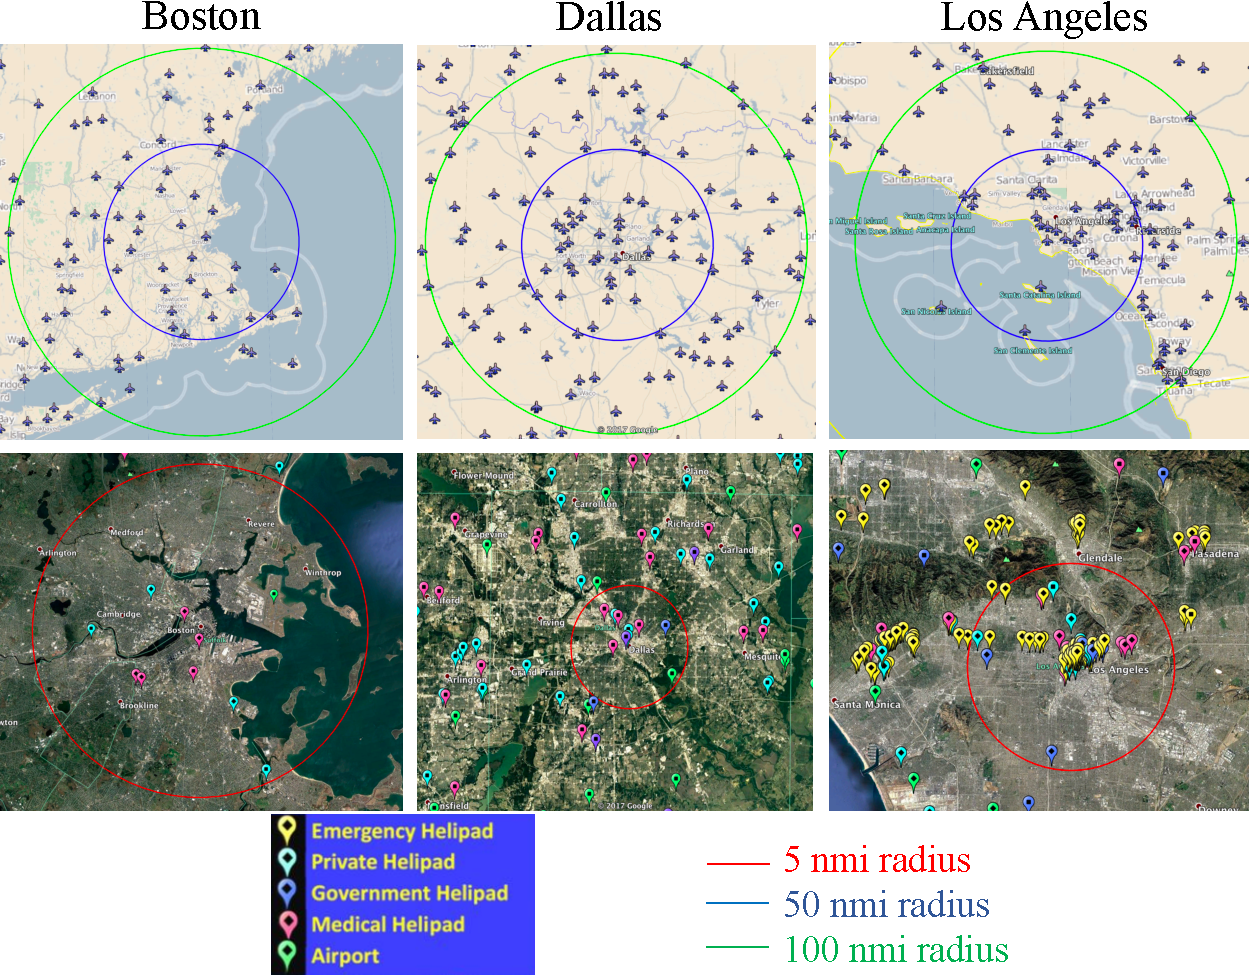
\includegraphics[width=1.0\textwidth]{available_inf.pdf}
    \caption{\textbf{Surface congestion surrounding major metropolitan areas drives the need for urban air transportation}}
	\label{f:inf_avail}
	\end{center}
\end{figure}

If significant new infrastructure investments are required in any case to make the UAM vision a reality, then the feasibility of the STOL UAM concept rests strongly on whether there are sufficient potential locations to build new takeoff and landing areas (TOLAs) in these urban cores.  Clearly, whether this is a feasible proposition is strongly dependent on how long of a runway is required.  At the scale of conventional commercial aircraft, with required runways lengths in the thousands of feet, it will infeasible to build substantial new infrastructure.  On the other end of the spectrum, VTOL aircraft maximize the number of potential infrastructure locations, although noise considerations may prove to be a significant limiting factor.  However, the trade space in between these two ends of the spectrum is poorly understood. Boston will therefore be used as an example case study to examine the effects of the runway length on feasible infrastructure locations.  This study is shown in Section V.   

\section{Vehicle Design Considerations and Key Enabling Technologies}
Historically, STOL aircraft make a number of design compromises to achieve short-field performance, the significance of which increase as the required runway length becomes shorter.  This section will discuss some of the key vehicle-level trades involved in designing an aircraft for short-field performance, and will discuss some of the ways that emerging electric aircraft technologies will offer improved performance over historical vehicles. 


\paragraph{Short Takeoff and Landing Considerations}
Figure ~\ref{f:takeoff} shows a simplified sketch of the aircraft during takeoff (top) and landing (bottom).  At a high level, the runway a vehicle operates off of must be equal to the larger of either the takeoff or landing distances.  To shorten the runway, both the takeoff and landing distances $S_{TO}$ and $S_{land}$ must be reduced.  The takeoff distance is a function of the time it takes the aircraft to reach a given liftoff speed $V_{LO}$, which is a multiple of the vehicle stall speed.  The stall speed is related to the high-level aircraft parameters by Equation ~\ref{e:stall}.  To reduce the takeoff distance, the vehicle design can be changed such that it reaches the liftoff speed faster by increasing the thrust, or the liftoff speed can be lower by decreasing the wing loading $W/S_{ref}$ increasing the wing $CL_{max}$.  These changes also serve to increase the climb angle $\gamma_{climb}$, which is desirable to minimize the time spent at low altitude. 
\begin{figure}[h!]
	\begin{center}
	\includegraphics[width=1.0\textwidth]{takeoff_fig.pdf}
    \caption{\textbf{Considerations for short takeoff and landing}}
	\label{f:takeoff}
	\end{center}
\end{figure}

\begin{equation}
    \label{e:stall}
    V_{\mathrm{TD,TO}} = 1.3V_{\mathrm{stall}} = \sqrt{\frac{2W_{\mathrm{MTO}}}{\rho S C_{L_{\mathrm{max}}}}}.
\end{equation}
Decreased $W/S_{ref}$ and increased $CL_{max}$ also help reduce the landing distance, since the reduce the touchdown speed $V_{TD}$, which is also scaled from $V_{stall}$.  Additionally, the landing distance may be shortened by increasing the drag after touchdown, either by wheel brakes, aerodynamic braking, or reverse thrust.  

For these reasons, compared to conventional takeoff and landing (CTOL) aircraft of the same size, STOL vehicles tend to be more lightly wing loaded, have high power-weight ratios, and have large and complex high-lift systems to increase $CL_{max}$ as much as possible.  To first order, high power-to-weight ratios and complex high-lift systems both add significant weight to the system, with second-order penalties on efficiency.  For a given aircraft, decreasing wing loading below its optimal value will limit the top speed of the vehicle, as well as making it more sensitive to wind gusts.  It will also increase the power required to cruise at a given speed, requiring additional fuel or batteries, or reducing range.  For these reasons, and since short field capability is not required at most airports, STOL aircraft have not widely adopted outside of the bush pilot community. 

The introduction of new electric aircraft technologies offer a variety of potential improvements over existing STOL aircraft, giving them significant advantages both in the UAM market and relative to current STOL vehicles.  This is similar to the way these technologies are being proposed to change vertical flight.  The following are the key technologies that are considered for an electric STOL (eSTOL) aircraft.  The impact of each technology will be assessed at a conservative baseline level, as well as a more optimistic advanced level to show the potential impact of technological improvements.  
\begin{wrapfigure}{R}{0.4\textwidth}
	\begin{center}
	\includegraphics{x-57.jpg}
    \caption{\textbf{The NASA X-57 will demonstrate the benefits of distributed electric propulsion for fixed-wing aircraft ~\cite{NASAWeb}}}
	\label{f:x57}
	\end{center}
\end{wrapfigure}
\paragraph{Distributed Electric Propulsion}
DEP is a collection of enabling technologies (high specific energy batteries, electric motors and controllers) that enable the replacement of a few large propulsors with many smaller ones.  The NASA X-57 shown in Figure ~\ref{f:x57} is an example of a fixed-wing DEP configuration currently being developed.   This novel propulsion system architecture allows optimization of different parts of the propulsion system for different phases of flight, which increases overall efficiency.  It also increased system redundancy, and most importantly for this application increases the effectiveness of the wing through blown lift (discussed below).  From a modeling perspective, it also allows cruise efficiency to be treated independently of takeoff power.  References ~\cite{StollDEP} and ~\cite{MooreDEP} discuss the benefits of DEP in more detail. 

\paragraph{Blown Lift}
Blown lift is a increases the effective wing lift coefficient through two main effects.  The first is the increase in effective dynamic pressure over the wing due to the accelerated propeller wake.  The second is the interaction between the propeller wake and the flaps, which turn the wake downward and produce an upwards force as a result. ~\cite{MooreDEP}.  Figure ~\ref{f:blown_lift} is from a NASA investigation into the effectiveness of blown lift. ~\cite{Deere}  It shows, for an X-57 like wing, that substantial increases in effective wing CL are possible.  As a conservative estimate, 4.0 was used as our baseline value of takeoff $CL_{max}$, and 5.0 for the advanced value.  
\begin{figure}[!h]
	\begin{center}
	\includegraphics[width = 1.\textwidth]{blown_lift_chart.pdf}
    \caption{\textbf{NASA studies show significant increases in $CL_{max}$ due to blown lift~\cite{study}}}
	\label{f:blown_lift}
	\end{center}
\end{figure}
From this figure it should be noted that the power required to achieve the high CL becomes quite high, especially in the landing configuration.  As discussed by Patterson ~\cite{Patterson2017}, this may limit the extent to which blown lift can be utilized during the approach phase of flight.  If the power required to achieve a high lift coefficient for a given vehicle exceeds the power required for a given approach angle (or level flight in the limit), then it is not useful for landing.  This effect may be offset by adding drag (spoilers, windmilling propellers) which would also have the beneficial effect of increasing approach angle; this is key vehicle-level trade study.  Based on the drag polars given in ~\cite{Deere}, an X-57 like aircraft would be limited to a $CL_{max}$ of 3.5 on approach without a high-drag system; for the purposes of this paper that is used as the baseline approach $CL_{max}$, and 4.5 is used for the advanced case.  

\paragraph{High Power Electric Motors}
Apart from their role as an enabling component of DEP, electric motors have two other useful capabilities for electric aircraft.  The first is the ability to be operated at power settings significantly higher than maximum continuous power for short periods of time.  Since high power is most important for a short time at takeoff, this effect could significantly minimize the weight penalty of a high-power propulsion system. ~\cite{Moore_Mis} Additionally, the rotation direction of these motors can be electrically reversed.  This is useful on braking to provide reverse thrust/massive drag at touchdown, which shortens landing distance without the weight penalty of dedicated thrust reversal systems.  

\paragraph{Advanced Flight Controls}
Autoland systems, which allow highly repeatable and precise landings, have become ubiquitous on commercial aircraft and have been proposed for emergency use in GA aircraft as well ~\cite{diana}.  In this context, a highly accurate autoland or landing guidance system could be used to reduce the margin of safety between the vehicle actual landing distance and required runway length.  Additionally, research is being done into autonomous post-stall landing maneuvers for fixed-wing micro air vehicles (MAVs) ~\cite{percher1} ~\cite{percher2} which could enable dynamic landing maneuvers near the vehicle stall speed.  Neither of these technologies are considered for the baseline technology variant, but are included in the advanced technology package.  All these technologies are summarized in Table ~\ref{t:tech}. 

% Table generated by Excel2LaTeX from sheet 'Sheet1'
\begin{table}[htbp]
  \centering
  \caption{Summary of eSTOL aircraft enabling technologies}
    \begin{tabular}{rrr}
          &       &  \\
    \midrule
          & \multicolumn{1}{p{14.915em}}{Baseline} & \multicolumn{1}{p{14.5em}}{Advanced} \\
    \midrule
    \multicolumn{1}{p{8.415em}}{D.E.P. } & \multicolumn{1}{p{14.915em}}{No loss of efficiency at cruise} & \multicolumn{1}{p{14.5em}}{No loss of efficiency at cruise} \\
    \multicolumn{1}{l}{\multirow{2}[0]{*}{Blown Lift}} & \multicolumn{1}{p{14.915em}}{Clmax Takeoff: 4.0} & \multicolumn{1}{p{14.5em}}{Clmax Takeoff: 5.0} \\
          & \multicolumn{1}{p{14.915em}}{Clmax Land: 3.5} & \multicolumn{1}{p{14.5em}}{Clmax Land: 4.5} \\
    \multicolumn{1}{l}{\multirow{2}[0]{*}{Electric Motor}} & \multicolumn{1}{p{14.915em}}{No additional power at takeoff} & \multicolumn{1}{p{14.5em}}{20\% additional power at takeoff} \\
          &       & \multicolumn{1}{p{14.5em}}{Reverse thrust on landing} \\
    \multicolumn{1}{p{8.415em}}{Advanced flight controls} & \multicolumn{1}{p{14.915em}}{Current required margins on stall speed and runway $V_{TD} = 1.3 V_{stall}$ $S_{runway} = 1.4*$max($S_{land}, S_{takeoff}$)} & \multicolumn{1}{p{14.5em}}{Reduction in required speed and runway margin ($V_{TD} = 1.1 V_{stall}$ and runway $S_{runway} = 1.2*$max($S_{land}, S_{takeoff}$)} \\
    \midrule
          &       &  \\
    \end{tabular}%
  \label{t:tech}%
\end{table}%


\section{Vehicle Feasibility}

A sizing study using Geometric Programming optimization was performed to understand how vehicle performance and design would be effected by short take offs and landings. 
This section describes the assumptions and equations used in the optimization model for vehicle size, cruise performance, and takeoff and landing distances.

Geometric programming was selected as a means of evaluating this trade space because of its speed and reliability.  
Geometric programming is a special type of convex, non-linear optimzation.\cite{gp}
Because it is convex, even GPs with thousands of variables can be solved quickly.\cite{gp}
Additionally, recent research has shown that GPs can be used to evaulate aircraft design trade spaces.\cite{burton_solar_2017}\cite{gpkit}


\subsection{Vehicle Model}

It is assumed that the aircraft is completely electric, replying on battery power for powered flight. 
The aircraft weight is comprised of the battery, payload, wing, motor, and structural weight,

\begin{equation}
    W_{\mathrm{MTO}} \geq W_{\mathrm{batt}} + N_{\mathrm{pax}}W_{\mathrm{pax}} + W_{\mathrm{wing}} + W_{\mathrm{motor}} + W_{\mathrm{struct}}
\end{equation}

where the motor, passenger, and structural weights are

\begin{align}
    W_{\mathrm{motor}} &\geq \frac{P_{\mathrm{shaft-max}}}{(P/W)_{\mathrm{motor}}} \\
    W_{\mathrm{pax}} &= 195 \mathrm{[lbf]} \\
    W_{\mathrm{struct}} &\geq W_{\mathrm{MTO}}f_{\mathrm{struct}}.
\end{align}

The battery weight is constrained by the range of the aircraft

\begin{equation}
    R \leq \frac{h_{\mathrm{batt}} W_{\mathrm{batt}} \eta_{\mathrm{elec}} V}{gP_{\mathrm{shaft}}}
\end{equation}

where the shaft power is 

\begin{equation}
    P_{\mathrm{shaft}} \geq \frac{TV}{\eta_{\mathrm{prop}}}
\end{equation}

The aircraft is assumed to be in steady level flight during cruise. 

The wing weight is composed of the skin, main spar and additional components

\begin{equation}
    W_{\mathrm{wing}} \geq W_{\mathrm{skin}} + W_{\mathrm{spar}} + W_{\mathrm{fadd}}
\end{equation}

The skin and structural elements are assumed to be carbon fiber.  
The wing spar configuration is a cap spar with unidirectional carbon fiber caps wrapped in a shear web as shown in Figure~\ref{f:capspar}.  

\begin{figure}[h!]
	\begin{center}
	\includegraphics[width=0.9\textwidth]{capspar.pdf}
    \caption{\textbf{Cross sectional view of a cap spar.}}
	\label{f:capspar}
	\end{center}
\end{figure}

The spar dimensions are sized such that the material stresses are not exceeded under a 3.5 g-load,

\begin{equation}
    \sigma_{\mathrm{CFRP}} \geq \frac{\mathcal{M}_{\mathrm{root}}}{S_{y_{\mathrm{spar}}}}
\end{equation}

The root wing moment $\mathcal{M}_{\mathrm{root}}$, is calculated assuming a distributed load along the wing span that scales with the local chord.\cite{bending}
A constant tapered wing is assumed.  
This wing sizing model leverages the GP wing sizing model used by Burton and Hoburg.\cite{burton_solar_2017} 

A simple drag model is used for the aircraft, 

\begin{equation}
    C_D \geq CDA + c_{d_p} + \frac{C_L^2}{\pi e AR}.
\end{equation}

where the profile drag coefficient $c_{d_p}(C_L, Re)$, is calculated from a representative wing polar. 
The combined drag and wing loading models allow the aspect ratio to be optimized, trading structural integrity with aerodynamic performance. 

\subsection{Takeoff and Landing Models}

The takeoff model was adapted from Raymer's takeoff equations to fit a GP compatible form.  Using equations of motion the takeoff state can be expressed

\begin{equation}
    T - D - \mu(W_{\mathrm{MTO}} - L) = \frac{W_{\mathrm{MTO}}}{g} \frac{dV}{dt}.
\end{equation}

This can be simplified to 
\begin{align}
    \frac{dV}{dt} &= g \left( \frac{T}{W_{\mathrm{MTO}}} - \mu \right) - \frac{g}{W_{\mathrm{MTO}}} \left( \frac{1}{2} \rho S V^2 (C_{D_g} - \mu C_{L_g})\right) \\
    \label{e:todiff}
    \frac{dt}{dV} &= \frac{1}{A-BV^2}
\end{align}

The takeoff ground run distance can then be expressed by taking the integral of Equation~\ref{e:todiff} to achieve

\begin{equation}
    \label{e:to}
    S_{\mathrm{TO}} = \frac{1}{2B} \ln{\frac{A}{A-BV^2}} 
\end{equation}

The natural log function can be approximated to make Equation~\ref{e:to} GP-comptible by 

\begin{equation}
    \ln{\frac{A}{A-BV^2}} \approx \num{5.6e-4} A^{-6.04} (BV^2)^{6.04} + 1.0 A^{-0.001} (BV^2)^{0.001} + \num{7.5e-4} A^{-1.276} (BV^2)^{1.275}
\end{equation}

with an average log error of 0.06\%.  The terms $A$, and $B$, are constrained by

\begin{align}
    \frac{T}{W_{\mathrm{MTO}}} &\geq \frac{A}{g} + \mu \\
    B &\geq \frac{g}{W_{\mathrm{MTO}}} \frac{1}{2} \rho S C_{D_g}
\end{align}

where the $\mu C_{L_g}$ term is neglected as a conservative approximation for $B$ to preserve GP-compatibility. 

The landing ground roll distance is calculated using conservation of energy, with the primary design variable being the loading deceleration factor, $N$.
This constraint will drive the wing loading down. 

\begin{equation}
    \label{e:sgr}
    S_{\mathrm{land}} \geq \frac{1}{2} \frac{V^2}{Ng} 
\end{equation}

where $N=1$ corresponds to a 1-g deceleration. 
The deceleration factor is a function of the technologies used to stop the aircraft and include, but are not limited to: brakes, reverse thrust from electric motors, and drag.  This was used instead of a more conventional braking model because, as discussed subsequently, these vehicles are driven primarily by landing constraints.  This creates an incentive to use some type of thrust reversal or dedicated braking thrust system to shorten the landing distance.  The details of this system are an important vehicle level design trade; the landing deceleration used in this system-level study becomes the design requirement for a future vehicle design effort. Passenger tolerance for negative deceleration may limit how high this target can be increased, but that requires future study.  
To understand how the g-loading constant varies with different amounts of reverse thrust, the ground roll and deceleration factor are calculate for the X-57 as an example case. 
Table~\ref{t:landingdecel} shows the deceleration loading factor for different amounts of reverse thrust. 

\begin{table}[H]
    \centering
    \caption{Landing Case for the X-57}
    \label{t:landingdecel}
    \begin{tabular}{lcc}
    \toprule
    \toprule
                                    & Ground          & Deceleration \\ 
                                    & Roll Distance   & Factor ($N$)\\ \hline
    Brakes only (dry)               &  925 [ft]       & 0.37  \\
    Brakes + 10\% reverse thrust    &  850 [ft]       & 0.4   \\
    Brakes + 50\% reverse thrust    &  625 [ft]       & 0.55  \\
    Brakes + 100\% reverse thrust   &  425 [ft]       & 0.73  \\
    \bottomrule
\end{tabular}
\end{table}

For both the landing and takeoff constraints it is assumed that the velocity has a 30\% margin above the stall velocity,
For the purposes of this study, deceleration corresponding to braking with a small amount of reverse thrust (.4g) was used for the conservative case, while a more powerful thrust reversal system (.7g) was used for the aggressive case. 
It is assumed that the the max lift coefficient is different for landing and takeoff.
Another 40\% margin is placed on the ground roll distance to determine runway length.  For this vehicle, balanced field length considerations were not considered as the loss of a single engine is only a small reduction in total thrust.  Additionally, takeoff distance over a 35ft obstacle was not considered since the focus is on determining the amount of physical infrastructure required.  Where appropriate (such as when the runway is located at ground level) the appropriate 35ft obstacle clearance will be added.  

\begin{align}
    S_{\mathrm{runway}} &\geq 1.4S_{\mathrm{TO}} \\
    S_{\mathrm{runway}} &\geq 1.4S_{\mathrm{land}} 
\end{align}

\subsection{Vehicle Trade Studies}

Using the geometric programming model of a STOL aircraft perviously described, tradeoffs between runway length and vehicle performance were evaulated.  The models consists of a 105 free variables and can be solved in approximately 0.1 seconds. 
Because aircraft scales with aircraft weight as a first order approximation, the objective function throughout is to minimize weight, $\min{(W_{\mathrm{MTO}})}$. 
Key parameters are defined in Table~\ref{t:params}.

\begin{table}[H]
    \centering
    \caption{Design Parameters}
    \label{t:params}
    \begin{tabular}{l c}
    \toprule
    \toprule
    Parameter                                   & Value         \\ \hline
    $S_{\mathrm{runway}}$                       & 300 [ft]      \\
    $\eta_{\mathrm{elec}}$                      & 0.9           \\
    $h_{\mathrm{batt}}$                         & 210 [Whr/kg]  \\
    $P_{\mathrm{spec}}$                         & 0.7136 [kW/N] \\
    $R$                                         & 100 [nmi]     \\
    $V_{\mathrm{min}}$                          & 100 [kts]     \\
    $C_{L_{\mathrm{max}}}$ (Landing)            & 3.5           \\
    $C_{L_{\mathrm{max}}}$ (TO)                 & 4.0           \\
    $N$                                         & 0.3g          \\
    $\eta_{\mathrm{prop}}$                      & 0.8           \\
    \bottomrule
\end{tabular}
\end{table}

To understand how passenger and runway requirements affect vehicle weight, the GP model was solved 30 times in 3.46 seconds.  
The results are shown in Figure~\ref{f:sw_mtow}, each point on the graph corresponding to a unique optimization solution or vehicle size.  
From this study it is observed that for runway lengths shorter than 250 ft are near infeasible for this set of parameters.  
It is also oberserved that the runway length is fairly insenstive to number of passengers.  

\begin{figure}[h!]
 \begin{subfigmatrix}{2}% number of columns
     \subfigure[\label{f:sw_mtow}Contours of number of passengers]{\includegraphics[]{sw_mtow.pdf}}
     \subfigure[\label{f:sw_mtowsens}Sensitivity to landing constraints]{\includegraphics[]{sw_mtowsens.pdf}}
 \end{subfigmatrix}
    \caption{\textbf{Trade space of aircraft weight, number of passengers and runway length.}}
 \label{f:sw_mt}
\end{figure}

To effectively shorten the field length it is important to know whether the vehicle size is driven by the landing or takeoff constraints. 
Qualitatively, the landing model has a direct effect on wing loading as shown in Equations~\ref{e:sgr} and~\ref{e:stall}.  
The takeoff model primarily effects the thrust to weight ratio but also has a small effect on the wing loading (Equation~\ref{e:to}). 
The effect of the thrust to weight ratio ($(T/W)$) and the wing loading ($(W/S)$) is shown in figure~\ref{f:to_land_arg}
The thrust to weight ratio drives the motor weight.  
The wing loading drives the wing size, which in turn drives the wing weight, drag and ultimately battery weight.  
This argument implies that the landing model would constrain the vehicle size. 

\begin{figure}[h!]
	\begin{center}
	\includegraphics[width=0.7\textwidth]{to_land_arg.pdf}
    \caption{\textbf{Effect of thrust to weight and wing loading ratios on vehicle size.}}
	\label{f:to_land_arg}
	\end{center}
\end{figure}

This hypothesis, that vehicle size is more constrained by landing than takeoff, can be confirmed by looking at the sensitivity to both the landing and takeoff models. 
The sensitivity to a variable in a geometric program is defined as the percentage change in the objective function for a 1\% change in that variable's value.  
Therefore, if the sensitivity to the landing constraints is greater in magnitude than the sensitivity to the take off constraints then the system is landing constrained.  
In figure~\ref{f:sw_mtowsens} the magnitude of sensitivity to the landing constraints is greater than the sensitivity to the takeoff constraints confirming that the aircraft is landing length driven. 
The sensitivity to the takeoff constraints is not zero because the takeoff model requires a thrust to weight ratio which determines the motor weight. 


\subsection{Requirement Trade Studies}

Because of the low wing loading required by the takeoff and landing models, the the optimum cruise speed of a STOL vehicle tends to be fairly slow.
Therefore, a minimum cruise speed requirement is imposed in the model

\begin{equation}
    V_{\mathrm{cruise}} \geq V_{\mathrm{min}}.
\end{equation}

The minimum speed requirement affects the amount of power draw and consequently the amount of batteries needed.  
This affects the ability to reach higher ranges and also increases the wing loading requiring longer runways.  
One way to achieve higher range or shorter runways is to decrease the required minimum speed during cruise.  
Conversely, flying faster requires shorter ranges or longer runways.
This trade off is shown in Figure~\ref{f:minspeed}.
The flat portion of the curves indicates that the aircraft is not constrained by the minimum cruise speed (i.e. that constraint is not active) because the optimum cruise speed for that set of requirements is faster than the minimum cruise speed. 

\begin{figure}[h!]
 \begin{subfigmatrix}{2}% number of columns
     \subfigure[\label{f:vweightR}Contours of range]{\includegraphics[]{vweightR.pdf}}
     \subfigure[\label{f:vweightS}Contours of runway length]{\includegraphics[]{vweightS.pdf}}
 \end{subfigmatrix}
 \caption{\textbf{Trade study between requirements of runway length, minimum speed and range.}}
 \label{f:minspeed}
\end{figure}

\subsection{Advanced Technology Trade Studies}

The previous section showed fundamental trade studies and trends for how runway length varies with performance.  
It is also possible to shorten runway length through advanced technology. 
As discussed previously, a number of technologies could help reduce the required runway length including power bursts from electric motors, reverse thrust on landing, advanced flight controls, and improved battery technology.  
The effect of these technology advances on required runway length can be observed by changing a few parameters from the baseline case and resolving the optimization model.
Table~\ref{t:techparams} compares the conservative parameters to the aggressive technology parameters that were assumed in the optimization model based off of the technologies discuessed in Table~\ref{t:techtable}. 

\begin{table}[H]
    \centering
    \caption{Advanced Technology Parameter Assumptions}
    \label{t:techparams}
    \begin{tabular}{l l c c}
    \toprule
    \toprule
    Technology                  & Parameter                         & Conservative Value  & Aggressive Value \\ \hline
    Battery improvements        & $h_{\mathrm{batt}}$               & 210 [Whr/kg]        & 300 [Whr/kg]\cite{batterytrend}\cite{seeo}     \\
    Motor power burst           & $(P/W)_{\mathrm{motor}}$          & 0.7136 [kW/N]       & 0.571 [kW/N]     \\
    Blown wing                  & $C_{L_{\mathrm{max}}}$ (Landing)  & 3.5                 & 4.5              \\
    Blown wing                  & $C_{L_{\mathrm{max}}}$ (TO)       & 4.0                 & 5.0              \\
    Reverse thrust              & Decleration Factor                & 0.4                 & 0.7              \\
    Advanced flight controls    & Runway margin                     & 40\%                & 20\%             \\
    Advanced flight controls    & Stall speed margin                & 30\%                & 10\%             \\
    \bottomrule
\end{tabular}
\end{table}

Understanding the extremes between the conservative case and a more aggressive case is useful in determining a feasible vehicle design and vehicle requirements. 
Figure~\ref{f:sw_mtt} shows the same trade study as figure~\ref{f:sw_mt}, but with the updated parameter values shown in Table~\ref{t:techparams}.

\begin{figure}[h!]
 \begin{subfigmatrix}{2}% number of columns
     \subfigure[\label{f:sw_mtowt}Contours of number of passengers]{\includegraphics[]{sw_mtowt.pdf}}
     \subfigure[\label{f:sw_mtowtsens}Sensitivity to landing constraints]{\includegraphics[]{sw_mtowtsens.pdf}}
 \end{subfigmatrix}
    \caption{\textbf{Trade space of aircraft weight, number of passengers and runway length for advanced technology assumptions.}}
 \label{f:sw_mtt}
\end{figure}

As observed in figure~\ref{f:sw_mtowt}, the advanced techonology assumptions allow for a much shorter runway than the baseline case showing that runways below even 100 ft might be possible. 
To understand which parameters have the largest effect on this trade study, each parameter can be varied one at a time from the baseline case. 
Figure~\ref{f:tech} show variations on the 5 passenger contour from figure~\ref{f:sw_mtow}. 

\begin{figure}[h!]
 \begin{subfigmatrix}{3}% number of columns
     \subfigure[\label{f:smtow_clmax}Contours of $C_{L_{\mathrm{max}}}$]{\includegraphics[]{smtow_clmax.pdf}}
     \subfigure[\label{f:smtow_gl}Contours of deceleration factor]{\includegraphics[]{smtow_gl.pdf}}
     \subfigure[\label{f:smtow_hbatt}Contours of battery specific energy]{\includegraphics[]{smtow_hbatt.pdf}}
 \end{subfigmatrix}
    \caption{\textbf{Trade space of aircraft weight, number of passengers and runway length for advanced technology assumptions.}}
 \label{f:tech}
\end{figure}

Note that increasing the maximum lift coefficient or the deceleration factor has no effect for higher runway lengths.  
This is because at higher runway lengths the size of the aicraft is constained by the range requirement but not the runway requirement. 
Increasing the battery specific energy however, is always beneficial because that lowers the battery weight which improves the whole system. 

\subsection{Point of Departure Vehicle}

A ``point of departure'' vehicle was sized for both the conservative case and aggressive case, whose parameter values are listed in Table~\ref{t:techparams}.  
Key variable values for both solutions are listed in Table~\ref{t:pod}.

\begin{table}[H]
    \centering
    \caption{Design Variables}
    \label{t:pod}
    \begin{tabular}{l c c}
    \toprule
    \toprule
    Parameter                   & Conservative Case  & Aggressive Case \\ \hline
    $W_{\mathrm{MTO}}$          & 2633 [lbf]         & 2010 [lbf] \\
    $W_{\mathrm{batt}}$         & 873 [lbf]          & 460 [lbf] \\
    $N_{\mathrm{pax}}$          & 5                  & 5  \\
    $AR$                        & 11                 & 10 \\
    $b$                         & 40 [ft]            & 30 [ft] \\
    $(W/S)$                     & 18 [lbf/ft$^2$]    & 23 [lbf/ft$^2$] \\
    $S_{\mathrm{runway}}$       & 400 [ft]           & 200 [ft] \\
    \bottomrule
\end{tabular}
\end{table}

One significant advantage this aicraft offers over an electric VTOL vehicle is the capacity to carry more passengers.  The proposed vehicle can carry 5 passengers, while electric VTOL vehicles are typically limited to 2.  
it is also noted that the runway length for the conservative case is 400 ft but runway lengths as short as 100 ft may be possible if all  of the advanced technology is used.  While all those benefits are unlikely to be realized in the near term, runway lengths of 200-300 feet are possibly if infrastructure availability requires it.  This is especially true of the speed or payload requirements are slightly reduced.  
This information can be used to inform infrastructure decisions.  
Figure~\ref{f:vehicle} shows a visualization of the point of departure vehicle.  
The design features a distributed electric propulsion system.  
Additionally, all the batteries are able to fit wings allowing for simpler fuselage configurations. 

\begin{figure}[h!]
 \begin{subfigmatrix}{2}% number of columns
     \subfigure[\label{f:sw_mtowt}]{\includegraphics[]{bottom_view_grey_bg.pdf}}
     \subfigure[\label{f:sw_mtowtsens}]{\includegraphics[]{iso_view_transparent_wing.pdf}}
 \end{subfigmatrix}
    \caption{\textbf{Point of departure vehicle drawing.}}
 \label{f:vehicle}
 \end{figure}

\section{Infrastructure Feasibility}
Infrastructure is another aspect of the system that drives the vehicle design. A range of feasible runway lengths is a requirement that flows from infrastructure and in turn defines what vehicle designs are also feasible. As previously discussed, there is a substantial amount of airport infrastructure located outside of urban centers; however within an urban center, much less airport or runway infrastructure exists. Therefore this Boston study will specifically consider feasible infrastructure within the urban center.  Key topics to address include what considerations drive the placement of STOLports, what are feasible location types, and how does infrastructure availability change with infrastructure type and required size. The goal in selecting locations for STOLport infrastructure is to be able to connect to existing transportation infrastructure within an urban center.
\paragraph{Site Considerations}
Site considerations are not driven solely by runway length. The minimum rectangular area upon which a STOLport can be built is defined by runway length as we well as room for taxiways, clearway requirements, and space for parking and charging stations. Clearway requirements are written in the FAA AC 150/5300 and are dependent on aircraft size and speed ~\cite{AC150}. For locations that may be space restricted, a STOLpad rather than a STOLport concept is possible, which would consist of only the bare minimum infrastructure and would not include space for considerations such as parking and charging stations. Site considerations are also dependent on VFR approach and departure paths and the need for obstacle avoidance. Obstacle avoidance is defined as a plane of a defined width at a given distance and height from the runway, through which no obstacle may protrude; obstacle avoidance definitions are also dependent on vehicle size and speed ~\cite{AC150}. The key drivers for site considerations are area available, which is more than solely runway length, and obstacle avoidance for approach and departure paths.\\
One other factor to consider when analyzing potential STOLport infrastructure is the weight capacity of the construction. Taking a look at a case study of Boston, there is currently five existing helipads on top of buildings within the city limits. The helipad construction allows for helicopters of maximum weight ranging from 10,000 to 22,000 pounds to land on the pads. This shows that with current construction materials and techniques, similar STOLports could be built to meet the landing requirements of the proposed Baseline (3180lb MTOW) and Advanced (2080lb MTOW) point of departure STOL vehicles.

\paragraph{Crosswind Mitigation}

An additional consideration for infrastructure availability is crosswind mitigation. In order to have a robust UAM system, wind should not be a prohibitive factor for operations. Specific considerations for the particular wind patterns of the city in question should be incorporated when deciding on infrastructure location. There are various techniques to mitigate for multiple wind directions. One way is to have conventional crosswind runways. A disadvantage for this is that it will require additional surface area for the STOLport, which could possibly reduce the amount of infrastructure available. To reduce the severity of this impact, the crosswind design could take credit for the headwind component inherent in triggering the switch to the crosswind runway. A rule of thumb says that take-off and landing distances are reduced by 1.5 $\%$  for each knot of headwind up to 20 knots ~\cite{Headwind}. An additional option would be to create a circular STOLport with the diameter of the required runway length. The runway heading could be set dynamically based on the prevailing winds. This would require more complex approach and departure procedures, 360-degree obstacle clearance, and portable charging stations. If the STOLport is built over linear pre-existing infrastructure such as highways and railways, an additional STOLport can be built nearby with a perpendicular orientation to serve the same geographic location when crosswind conditions exist. Lastly, if barges are used as the STOLport then they could be moored to allow for rotation into the wind. This would require an increased footprint in the waterways which needs to be deconflicted with boating channels.
In addition to infrastructure design, the eSTOL vehicle design could also be used to mitigate crosswind landings. A larger vertical stabilizer or increased control surface could increase the safe crosswind strength on landing. The design could also incorporate specific adjustments to the landing gear to facilitate higher crosswind landings, such as rotating landing gear, which would allow the nose of the aircraft to remain into the wind all the way through touchdown. One additional design consideration would be to introduce advance controls or maneuvers to allow for safe crosswind landings. With advances happening rapidly with high-precision approach and landing guidance, crosswind landings can be mitigated through automation.

\paragraph{Logan Airport Considerations}
One of the main locations for a STOLport would be at major hub airports. In Boston, Logan International Airport would act as both a connection to nodal transportation for the UAM network and a constant supply of passengers requesting on-demand mobility. Logan averages 1,062 operations (take-offs and landings) per day ~\cite{LoganStats}. According to Massport, Logan can accommodate 120 operations per hour during ideal weather conditions. This number is reduced to 60 operations per hour during poor weather conditions ~\cite{LoganOps}. While this shows that there is some excess capacity for ATC at Logan, as the UAM market scales additional deconfliction measures need to be implemented.
STOL aircraft introduce novel uses of runways at pre-existing airfields. With landings of less than 500 feet, STOL aircraft could possibly have the opportunity to land to vacant runways and taxiways based on the current take-off/landing configuration. STOL aircraft could also receive landing clearance to land and hold short of active runways with their short landing capability. The ideal situation however would be to establish a parallel STOL runway greater than 4,300 feet from the active runway to allow for independent simultaneous operations to the current traffic pattern. Logan Airport has pre-existing infrastructure of runways and taxiways that would facilitate a STOL runway of at least 500 feet for each of the four standard wind configurations as shown in Figure ~\ref{f:logan}.
\begin{figure}[h!]
	\begin{center}
	\includegraphics[width=1.0\textwidth]{Logan Independent Ops.pdf}
    \caption{\textbf{STOL capability allows for additional takeoff and landing operations at major airports.}}
	\label{f:logan}
	\end{center}
\end{figure}

\paragraph{Feasible Locations}
A network of notional sites within Boston was designed with the previous considerations in mind. The network of notional sites is shown in Figure ~\ref{f:nsites}. Within the network there are four types of possible STOLport locations, which are also shown in Figure ~\ref{f:nsites}. The four types of locations to place a STOLport are on top of a building, over a highway or railway, on a barge over a body of water, or on the ground. Visualizations for the four types of STOLport locations are shown in Figure ~\ref{f:svis}. The barge location shows a runway and possible space for charging stations.  The highway or railway location shows a runway on an elevated structure, with a ramp for the aircraft to taxi down to a lower level with charging stations. The building location shows the possibility for crosswind runways depending on the are available, and space for charging stations are also shown. The ground location is similar to the building location with crosswind runways depending on the area available and charging stations again shown. The network of notional sites identified accounting for previously discussed considerations included building locations, highway or railway locations, barge locations, and ground locations.
\begin{figure}[h!]
	\begin{center}
	\includegraphics[width=1.0\textwidth]{2 Notional Sites.pdf}
    \caption{\textbf{Notional sites for STOLport locations}}
	\label{f:nsites}
	\end{center}
\end{figure}
\begin{figure}[h!]
	\begin{center}
	\includegraphics[width=1.0\textwidth]{3 STOLport Visualizations.pdf}
    \caption{\textbf{STOLport placement options}}
	\label{f:svis}
	\end{center}
\end{figure}
\paragraph{Scaling}
Buildings are the type of infrastructure location that is most dependent on runway length. Considerations for scaling an infrastructure network do vary between the types of locations. At highway and railway locations, placing any length of runway is fairly easy because the length of highways and railways far exceeds the length of STOLport runways. For highways and railways, possible scaling challenges include the fact that highway and railway infrastructure is limited in downtown areas due to tunnels. For barges, many major cities are located by large bodies of water which allows for much available area in order to scale the number of barge locations. However barges must consider ways to connect to the shore and avoiding shipping lanes. Scaling a network of ground infrastructure locations is not really feasible in an urban center aside from already existing airports. Buildings are generally widely available within an urban center, however buildings will require shorter runway lengths compared to the other locations because of limited rooftop area. Building STOLport locations are the type of location that is most dependent on runway length.
	GIS building footprint data was analyzed in order to understand how building infrastructure varies with runway length. Again, buildings are the type of STOLport location most dependent on runway length, as discussed in the previous paragraph. GIS data provides the footprints of buildings in a city ~\cite{GIS_MA}~\cite{GIS_CA}. Based on this GIS data, if at least one side of the building footprint was as long as a given runway length, then the footprint was counted as a possible building. Figure ~\ref{f:heatmap} shows heat maps created using the building footprint GIS data for Boston and Los Angeles. The heat maps show that the possible buildings for different runway lengths are distributed throughout the city making it possible to scale an infrastructure network that is not all concentrated at one location. Using the same method of counting possible buildings from the GIS building footprint data, Figure ~\ref{f:hist} shows data trends of possible buildings as a function of runway length in order to provide insight into the manner in which the number of available buildings varies with runway length. For runway lengths of 400-600 feet, the number of possible buildings does allow for designing a network STOLport locations to be feasible. Runway lengths of 300 feet or less allow for a significant increase in the number of possible building locations for STOLports. The trend is that as runway length decreases, the number of possible buildings for STOLports exponentially increases.

\begin{figure}[h!]
	\begin{center}
	\includegraphics[width=1.0\textwidth]{4 Building Heat Maps.pdf}
    \caption{\textbf{Notional sites for STOLport locations}}
	\label{f:heatmap}
	\end{center}
\end{figure}
\begin{figure}[h!]
	\begin{center}
	\includegraphics[width=1.0\textwidth]{5 Building Histograms.pdf}
    \caption{\textbf{STOLport placement options}}
	\label{f:hist}
	\end{center}
\end{figure}

\section{Key Challenges and Risks}
There are several key challenges and risks that are inherent to the STOL UAM network that require further effort to understand more fully.    
\paragraph{Crosswinds} While there are several effective strategies for dealing with crosswinds, the relative effectiveness of each and their effect on network density requires further investigation.  This is likely to vary from city to city, based on the prevalent local wind conditions.  Additionally, the effect of crosswind considerations on vehicle design is an important part of the trade space, especially for these low-speed vehicles.  
\paragraph{Deconfliction with large-scale commercial operations}
This is a risk present for any UAM network, but operations in the vicinity of a busy hub airport like Boston Logan require careful ATC coordination to ensure safe separation between landing commercial aircraft and UAM vehicles.   This is especially true for UAM aircraft landing at or near large hub airports. 
\paragraph{Passenger Comfort} STOL operations require significant accelerations and decelerations on takeoff and landing, and the lightly wing loaded vehicles have high gust susceptibility. All of these factors may negatively impact passenger comfort.  Gust-damping systems similar to those found on large commercial aircraft may be used.  Passenger comfort is difficult to quantify; where this limits the vehicle design needs to be investigated in more detail.
\paragraph{Reverse thrust systems} There is a clear benefit to having a reverse thrust system for a STOL vehicles.  However, it is unclear how effective reversing propeller rotation direction would be, or if more effective (but heavy) variable pitch props are required.  The effects of wet runways also need to be considered.  
\paragraph{Noise and Community overflight} It is unclear that the noise levels generated by these vehicles will be low enough to allow widespread operations over noise-sensitive areas. More detailed modeling is required to understand the exact noise impact of these types of vehicles, relative to both eVTOL configurations and the annoyance threshold of the surrounding populations.  It is also recognized that the shallow (relative to an eVTOL) approach and departure angles mean that surrounding communities might experience more overflight below 500ft.  However, with the blown flaps and high T/W, very steep departure angles are possible, which may give total noise exposure similar to eVTOLs.  On approach, the power setting will be low so the primary negative effects of overflight (noise) should be reduced.  This requires more in-depth work. 

\section{Conclusion}
This analysis has showed that eSTOL aircraft are a feasible option for a UAM network, with significant advantages relative to vehicle payload and certification risk.  Vehicle runway lengths as short as 200-300 ft are shown to be feasible with current technologies, although a cruise speed reduction or some advanced technology may be required to achieve 200ft.   Runway lengths above 400ft are readily achievable for eSTOL aircraft. 
Possible types of locations for STOLports identified in this study include on top of buildings, over highways and railways, on barges, or on the ground of existing airports. Building infrastructure is the type of location most dependent on runway length. The STOLport locations can support runway lengths of 400 to 600 feet. If a vehicle is able to land in a runway of 300 feet or less, then the number of possible STOLport locations exponentially increases. Landing in a runway length of 500 feet or less could allow for novel operations at existing major airports. The results of the infrastructure study indicate that it is possible to design a STOLport network in an urban center.
STOL aircraft offer a near-term pathway to implementing a UAM network, allowing a company to capture early market share and start developing the operational knowledge of how to conduct these types of operations in the existing ATC environment.  STOL is a low-risk way to advance, test, and refine the UAM concept and all underlying technologies and operational infrastructures.  
\bibliography{biblibrary}
\bibliographystyle{aiaa}

\end{document}

